\chapter{Durchführung}

\label{chap:Durchführung}

Für die Kalibrierung und die Probenvermessung müssen verschiedene Reaktionslösungen angesetzt werden, die einerseits die Matrixeinflüsse verhindern und andererseits für die Farbreaktion benötigt werden. Im folgenden Kapitel sind die verwendeten Chemikalien und Geräte aufgelistet, sowie der genaue Arbeitsablauf gemäß der Vorschrift aus dem Buch Lebensmittelanalytik~\cite{Lebensmittelanalytik} beschrieben.

\section{Verwendete Chemikalien}

Um störende Matrixbestandteile der Honigproben vorab zu entfernen, werden die Carrez-Lösungen I und II benötigt. Die für die Farbreaktion verwendeten Reaktionslösungen können im Chemikalienhandel erworben werden. Dies gilt ebenfalls für die Reinsubstanz HMF, die für die Kalibrierlösungen und die Aufstockung benutzt wird. In der nachfolgenden Tabelle \ref{tab:Chemikalienliste} sind alle benötigten Chemikalien aufgelistet.

\begin{table}[htbp]
    \centering
        \caption{Chemikalienliste}
        \begin{tabular}{L{0.18\linewidth}|C{0.13\linewidth}|C{0.1\linewidth}|c|c|c} 
            Chemikalie & CAS/ Artikel-Nr. & Gefahren-symbol & Reinheit & Hersteller & Lot-Nr.\\
            \hline
            Hydroxymethyl-furfural & 67-47-0 & 
\includegraphics{../Bilder/Ausrufezeichen.jpg} & 97\% & Alfa Aesar & 10189124\\
            \hline
            p-Toluidin-lösung & 18686.2700 & 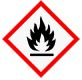
\includegraphics{../Bilder/Flamme.jpg} 
\includegraphics{../Bilder/Gesundheitsgefahr.jpg} 
\includegraphics{../Bilder/Ausrufezeichen.jpg} & 100g/L & Bernd Kraft & 1632697\\
            \hline
            Barbitursäure-lösung & 18685.2700 & - & 5g/L & Bernd Kraft & 1632696\\
            \hline
            Kaliumhexa-cyanoferrat-(II)-Trihydrat & 14459-95-1 & - & $\geq99\%$ & Sigma-Aldrich & SZBC2230V\\
            \hline
            Zinkacetat-Dihydrat & 5970-45-6 & 
\includegraphics{../Bilder/Ausrufezeichen.jpg} 
\includegraphics{../Bilder/Umwelt.jpg} & $\geq99,5\%$ & Merck & A0180402 142\\
            \hline
            VE-Wasser & & & & &
        \end{tabular}
    \label{tab:Chemikalienliste}
\end{table}

\begin{figure}[htbp]
    \centering
        \subfigure[p-Toluidinlösung]{
    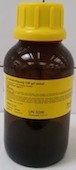
\includegraphics[]{../Bilder/20150504_140919.jpg}}
        \subfigure[Barbitursäurelösung]{
        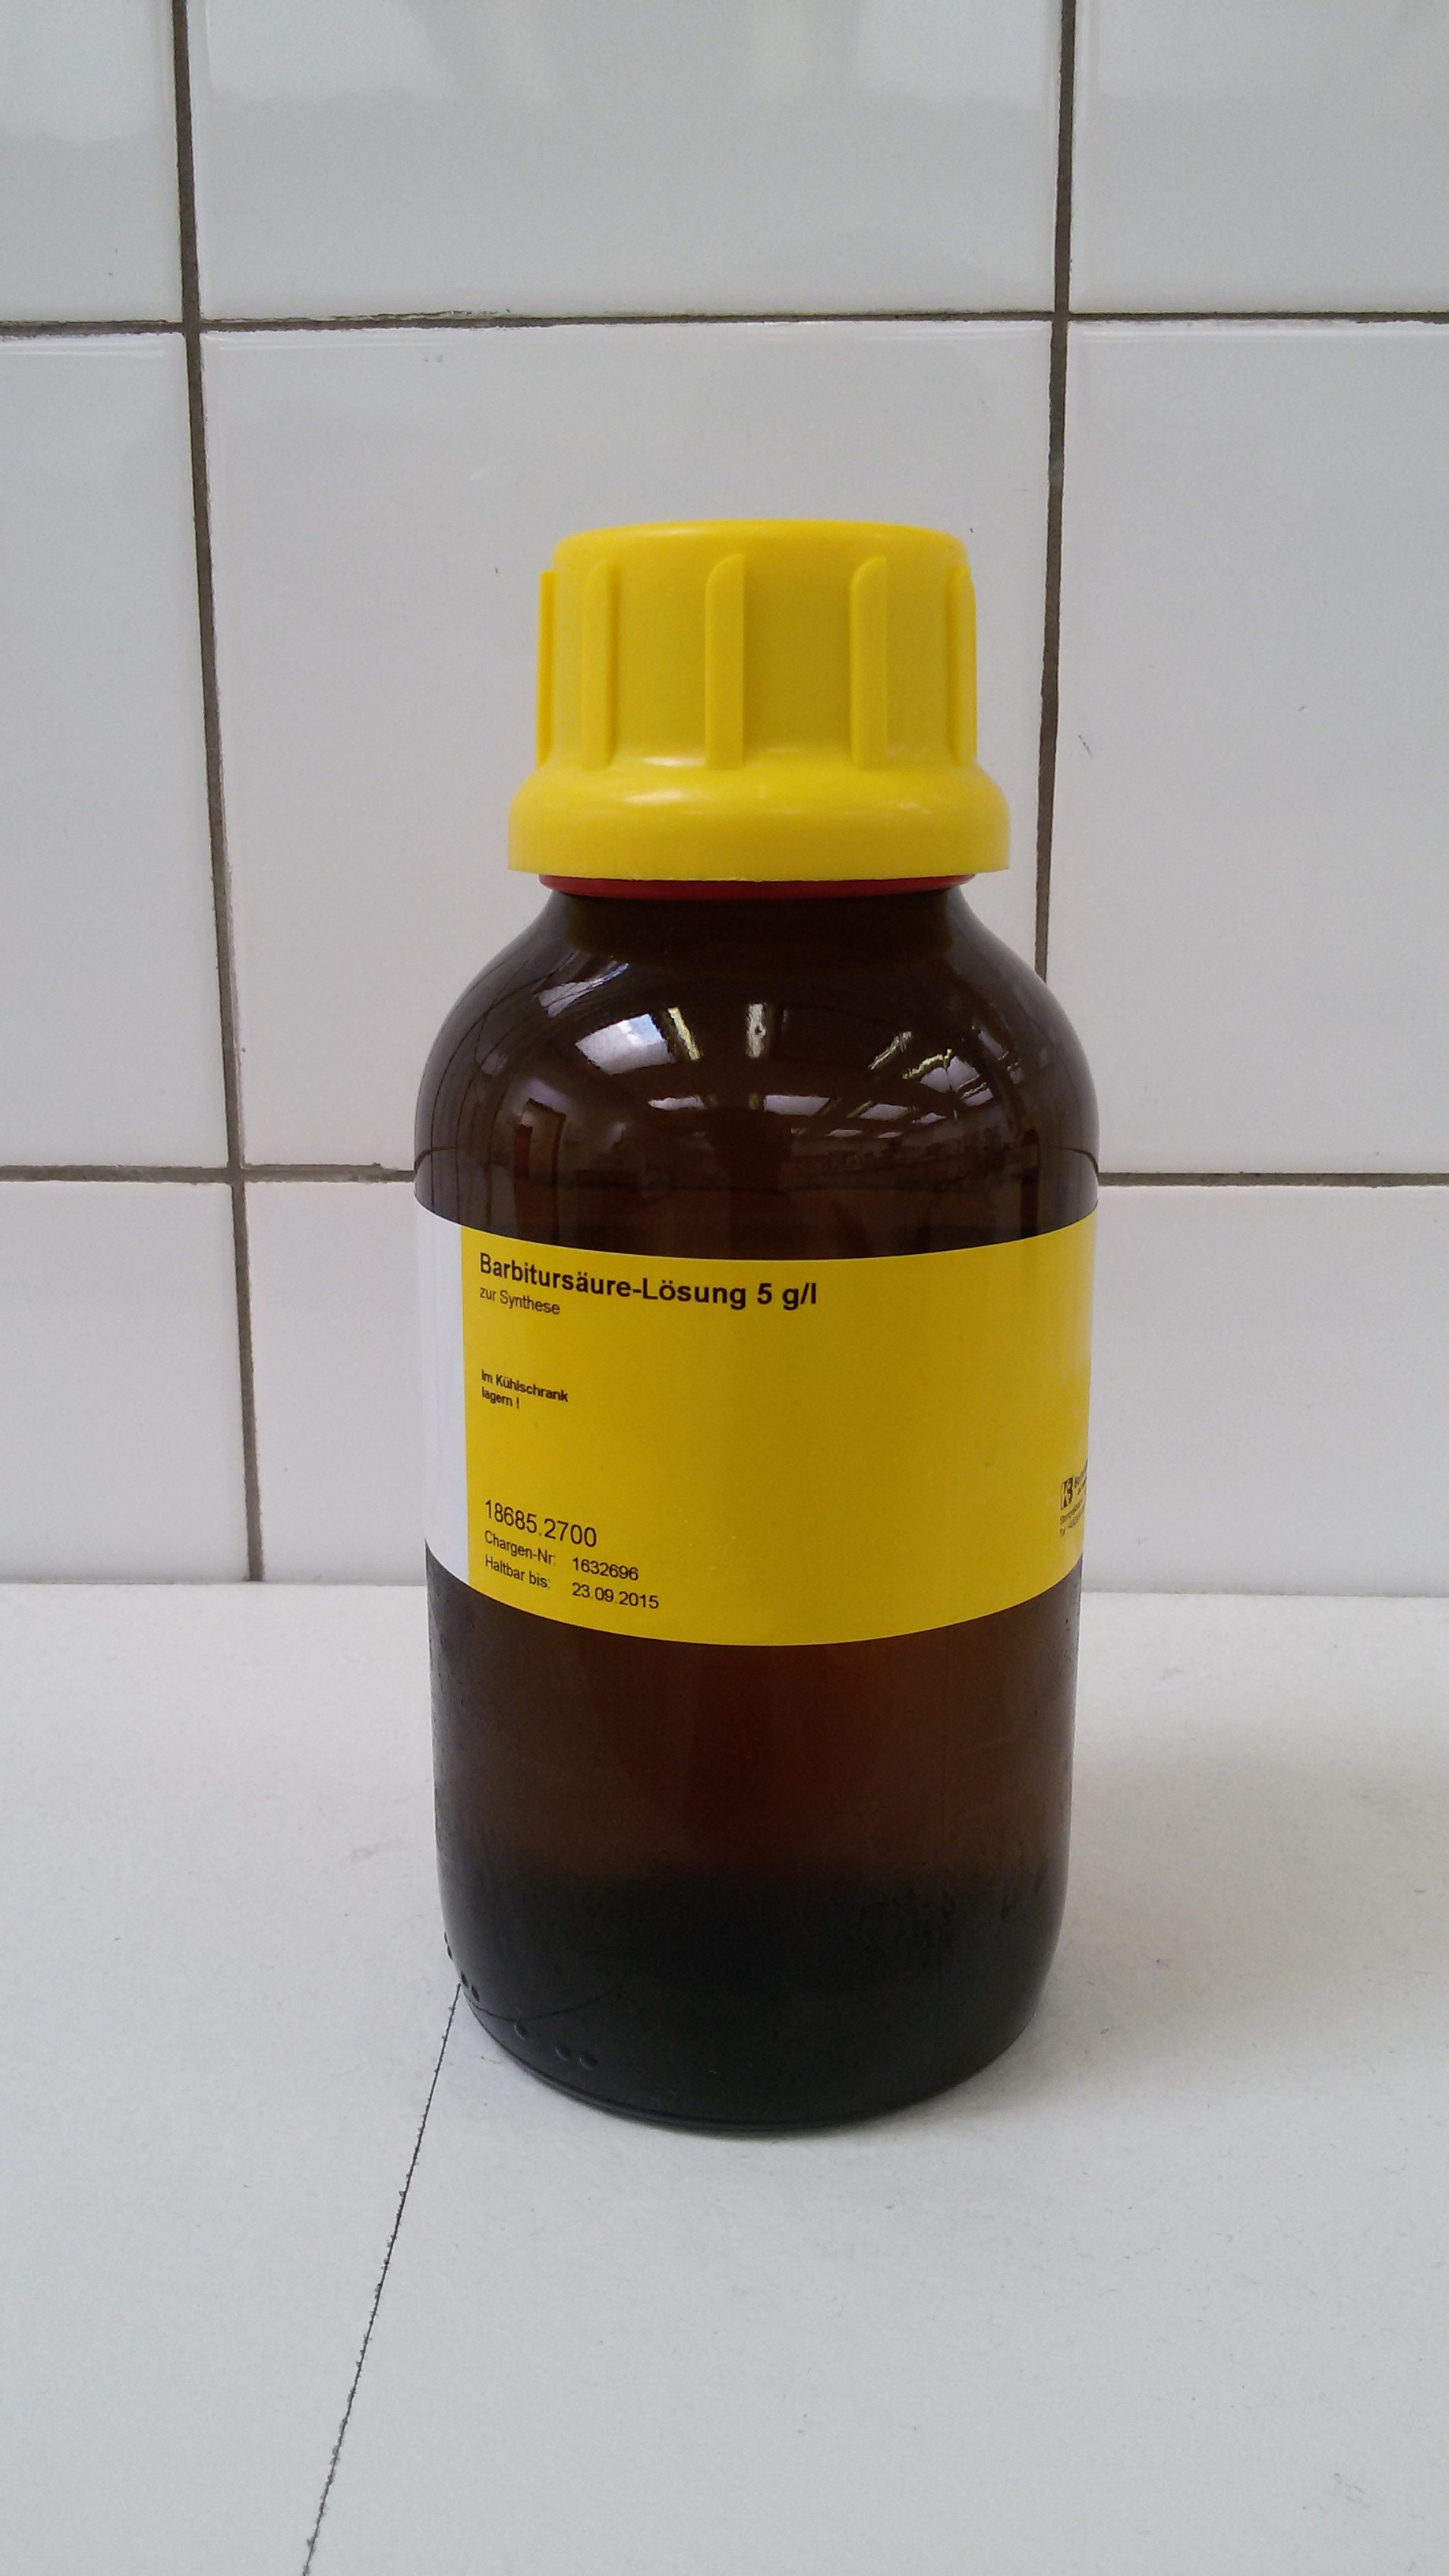
\includegraphics[]{../Bilder/20150504_140946.jpg}}
        \subfigure[\small Kaliumhexa-cyano-ferrat-(II)-Trihydrat]{
        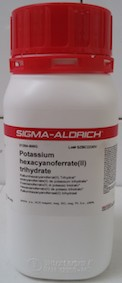
\includegraphics[]{../Bilder/20150504_141221.jpg}}
        \subfigure[Zinkacetat-Dihydrat]{
        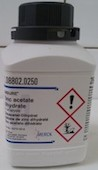
\includegraphics[]{../Bilder/20150504_141229.jpg}}
    \caption{Verwendete Chemikalien}
    \label{fig:Chemikalien}
\end{figure}

Die Sicherheitsdatenblätter sind in Anhang 4 - 8 zu finden.

\section{Verwendete Geräte}

Für die Probenvorbereitung und um die verschiedenen Lösungen herzustellen, werden diverse Laborgeräte verwendet. Diese sind in der folgenden Tabelle \ref{tab:Geräteliste} zusammengefasst.

\begin{table}[htbp]
    \centering
        \caption{Geräteliste}
        \begin{tabular}{l|C{0.25\linewidth}|c|c|c} 
            Anzahl & Gerät & Volumen in mL & Genauigkeit & Auslaufzeit\\
            \hline
            16 & Messkolben & 10 & A (+/- 0,040mL) & \\
            \hline
            8 & Messkolben & 50 & A (+/- 0,060mL) & \\
            \hline
            4 & Messkolben & 100 & A (+/- 0,100mL) & \\
            \hline
            4 & Vollpipetten & 1 & AS (+/- 0,006mL) & EX\\
            \hline
            2 & Vollpipetten & 2 & AS (+/- 0,010mL) & EX + 15s\\
            \hline
            1 & Vollpipetten & 5 & AS (+/- 0,015mL) & EX + 15s\\
            \hline
            1 & Vollpipetten & 10 & AS (+/- 0,02mL) & EX + 15s\\
            \hline
            1 & Vollpipetten & 20 & AS (+/- 0,03mL) & EX + 15s\\
            \hline
            1 & Messzylinder & 25 & & \\
            \hline
            diverse & Bechergläser & & & \\
            \hline
            1 & Wägeschiffchen & & & \\
            \hline
            1 & Analysenwaage Sartorius M-pact AX224 & max. 120g & d=0,1mg & 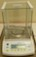
\includegraphics{../Bilder/20150504_140748.jpg}\\
            \hline
            1 & UV/VIS-Spektralphotometer Varian Cary® 50 & & & \\
            \hline
            1 & Präzisions-Küvette aus opt. Spezialglas & d=10mm & & \\
        \end{tabular}
    \label{tab:Geräteliste}
\end{table}


\section{Proben}

Es werden acht verschiedene Honige, ein Zuckerrübensirup und eine Invertzuckermischung vermessen. Die folgende Tabelle \ref{tab:Probenliste} zeigt die Probendetails.

\begin{table}[htbp]
    \centering
    \caption{Probenliste}
        \begin{tabular}{C{0.1\linewidth}|C{0.18\linewidth}|c|c|C{0.2\linewidth}|c} 
            Proben-nummer & Probe & Hersteller & Ablaufdatum & Herkunft & Lot-Nr.\\
            \hline
            1 & Flotte Biene Frühlings-blütenhonig & Langnese & 12.2016 & EU-Länder & LM41222\\
            \hline
            2 & Flotte Biene Gebirgs-blütenhonig & Langnese & 09.2016 & Nicht-EG-Länder & LI40946\\
            \hline
            3 & Sommer-blütenhonig & Vom Land & 06.2015 & EG- und Nicht-EG-Länder & L3442714\\
            \hline
            4 & Blütenhonig & Goldland & 03.2015 & EG- und Nicht-EG-Länder & LC40341\\
            \hline
            5 & Mexico & Biophar & 10.2016 & Mexiko & B582725\\
            \hline
            6 & Ägäis & Breitsamer & 07.2016 & Ägäis-Türkei & L4043131\\
            \hline
            7 & Waldhonig & Breitsamer & 10.2016 & Italien, Tschechien & L5644211\\
            \hline
            8 & Zuckerrüben-sirup & Grafschafter & 12.2017 & - & -\\
            \hline
            9 & Winterfutter & Imker B. Hahl & - & Walldorf, Deutschland & -\\
            \hline
            10 & Invertzucker & Pati-Versand.de & 09.2016 & - & 42090.58\\
        \end{tabular}
        \label{tab:Probenliste}
\end{table}

\begin{figure}[htbp]
    \centering
        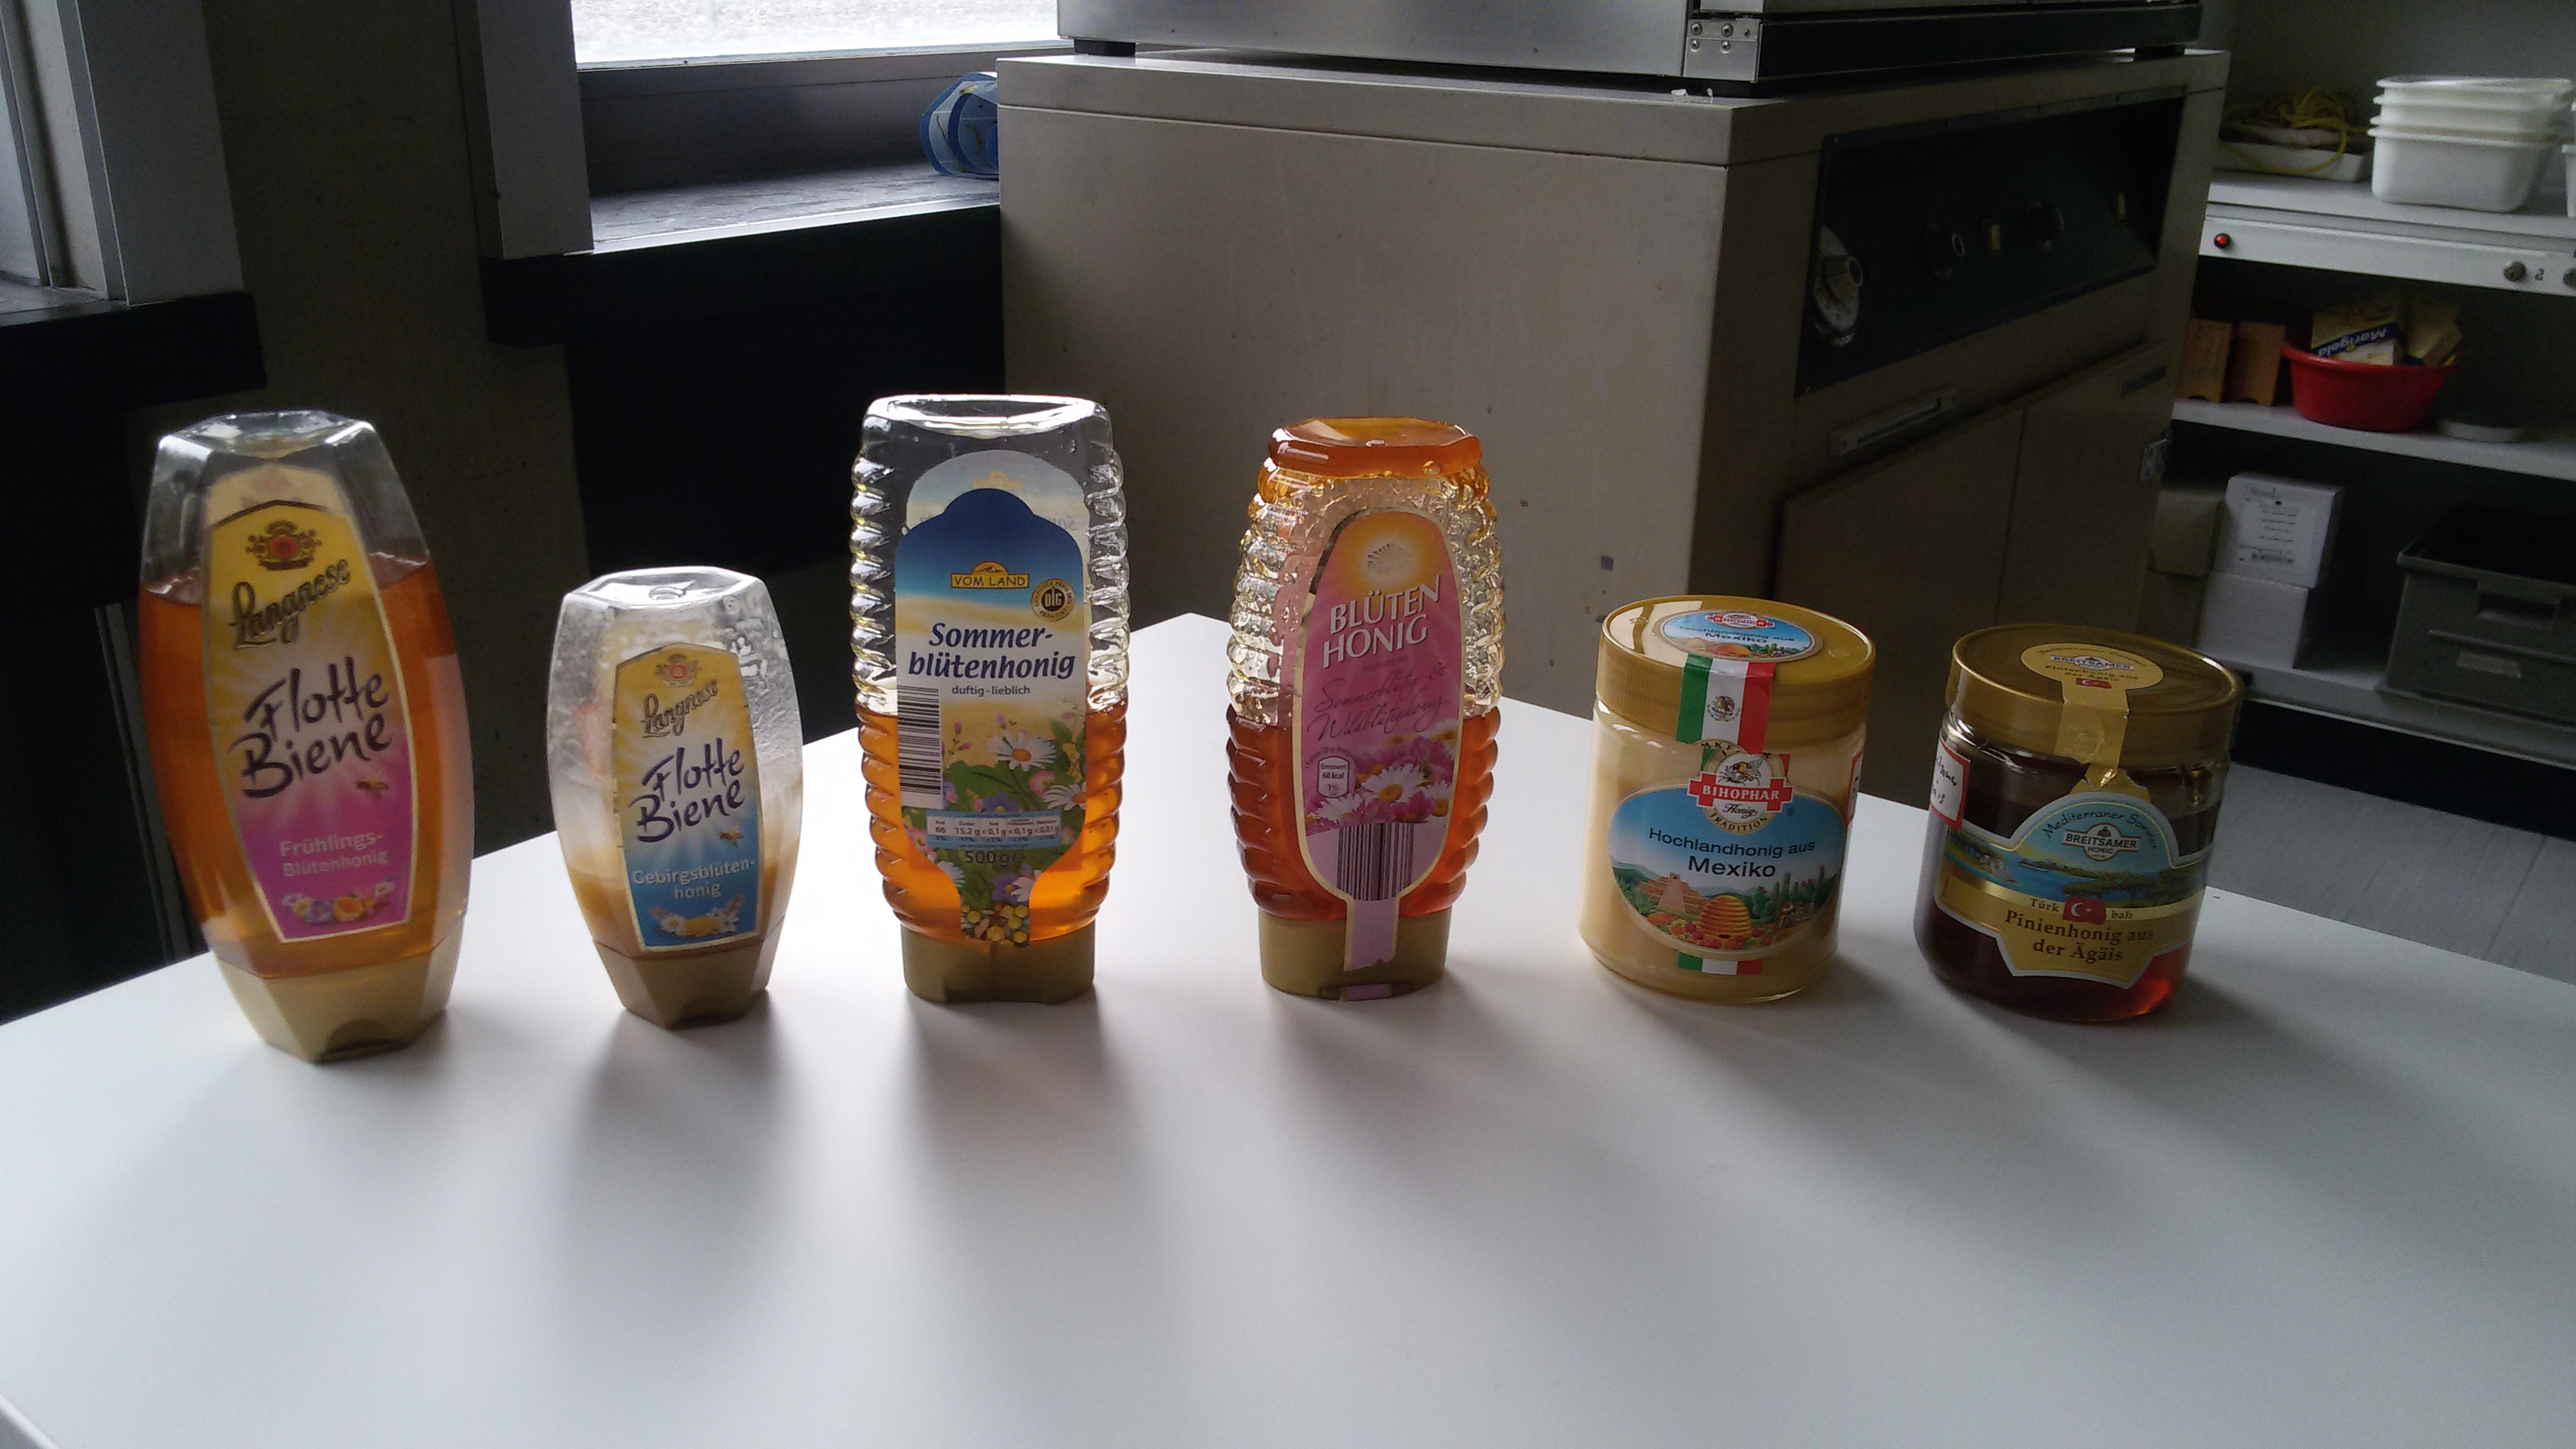
\includegraphics[width=1.00\textwidth]{../Bilder/20150416_183117.jpg}
    \caption{Übersicht der ersten sechs Honigproben}
    \label{fig:Honigproben}
\end{figure}


\section{Ansetzen der Reaktionslösungen}

Für die Probenaufbereitung werden zwei Carrez-Lösungen benötigt.\\ 
Für die Carrez-Lösung I wird am ersten Praktikumstag 15,1805g Kaliumhexacyanoferrat in einen 100mL Messkolben eingewogen, mit Wasser gelöst und bis zur Ringmarke aufgefüllt.\\ 
Die Carrez-Lösung II wurde zweimal angesetzt, da nach einer Woche Lagerung feste Partikel im Messkolben gefunden wurden. Am ersten Praktikumstag wurde für die Carrez-Lösung II 30,1485g Zinkacetat in einen 100mL Messkolben eingewogen, mit Wasser im Ultraschallbad gelöst und bis zur Ringmarke aufgefüllt. Da sich das Zinkacetat schlecht auflöste, wurde die Lösung beim zweiten Ansetzen am dritten Praktikumstag leicht erwärmt. Für die zweite Lösung wurde 30,0504g Zinkacetat eingewogen.\\ 
Die p-Toluidinlösung und die Barbitursäurelösung mussten nicht angesetzt werden, da sie in der benötigten Konzentration zur Verfügung standen. In der p-Toluidinlösung waren eine Woche nach Anbruch Feststoffpartikel enthalten.

\section{Ansetzen der Stammlösungen}

Für die Kalibrierreihe werden zwei Stammlösungen mit unterschiedlicher HMF-Konzentration angesetzt. Die Berechnung der benötigten Einwaagen befindet sich in Kapitel \ref{chap:Planung}.

\begin{figure}[htbp]
    \centering
        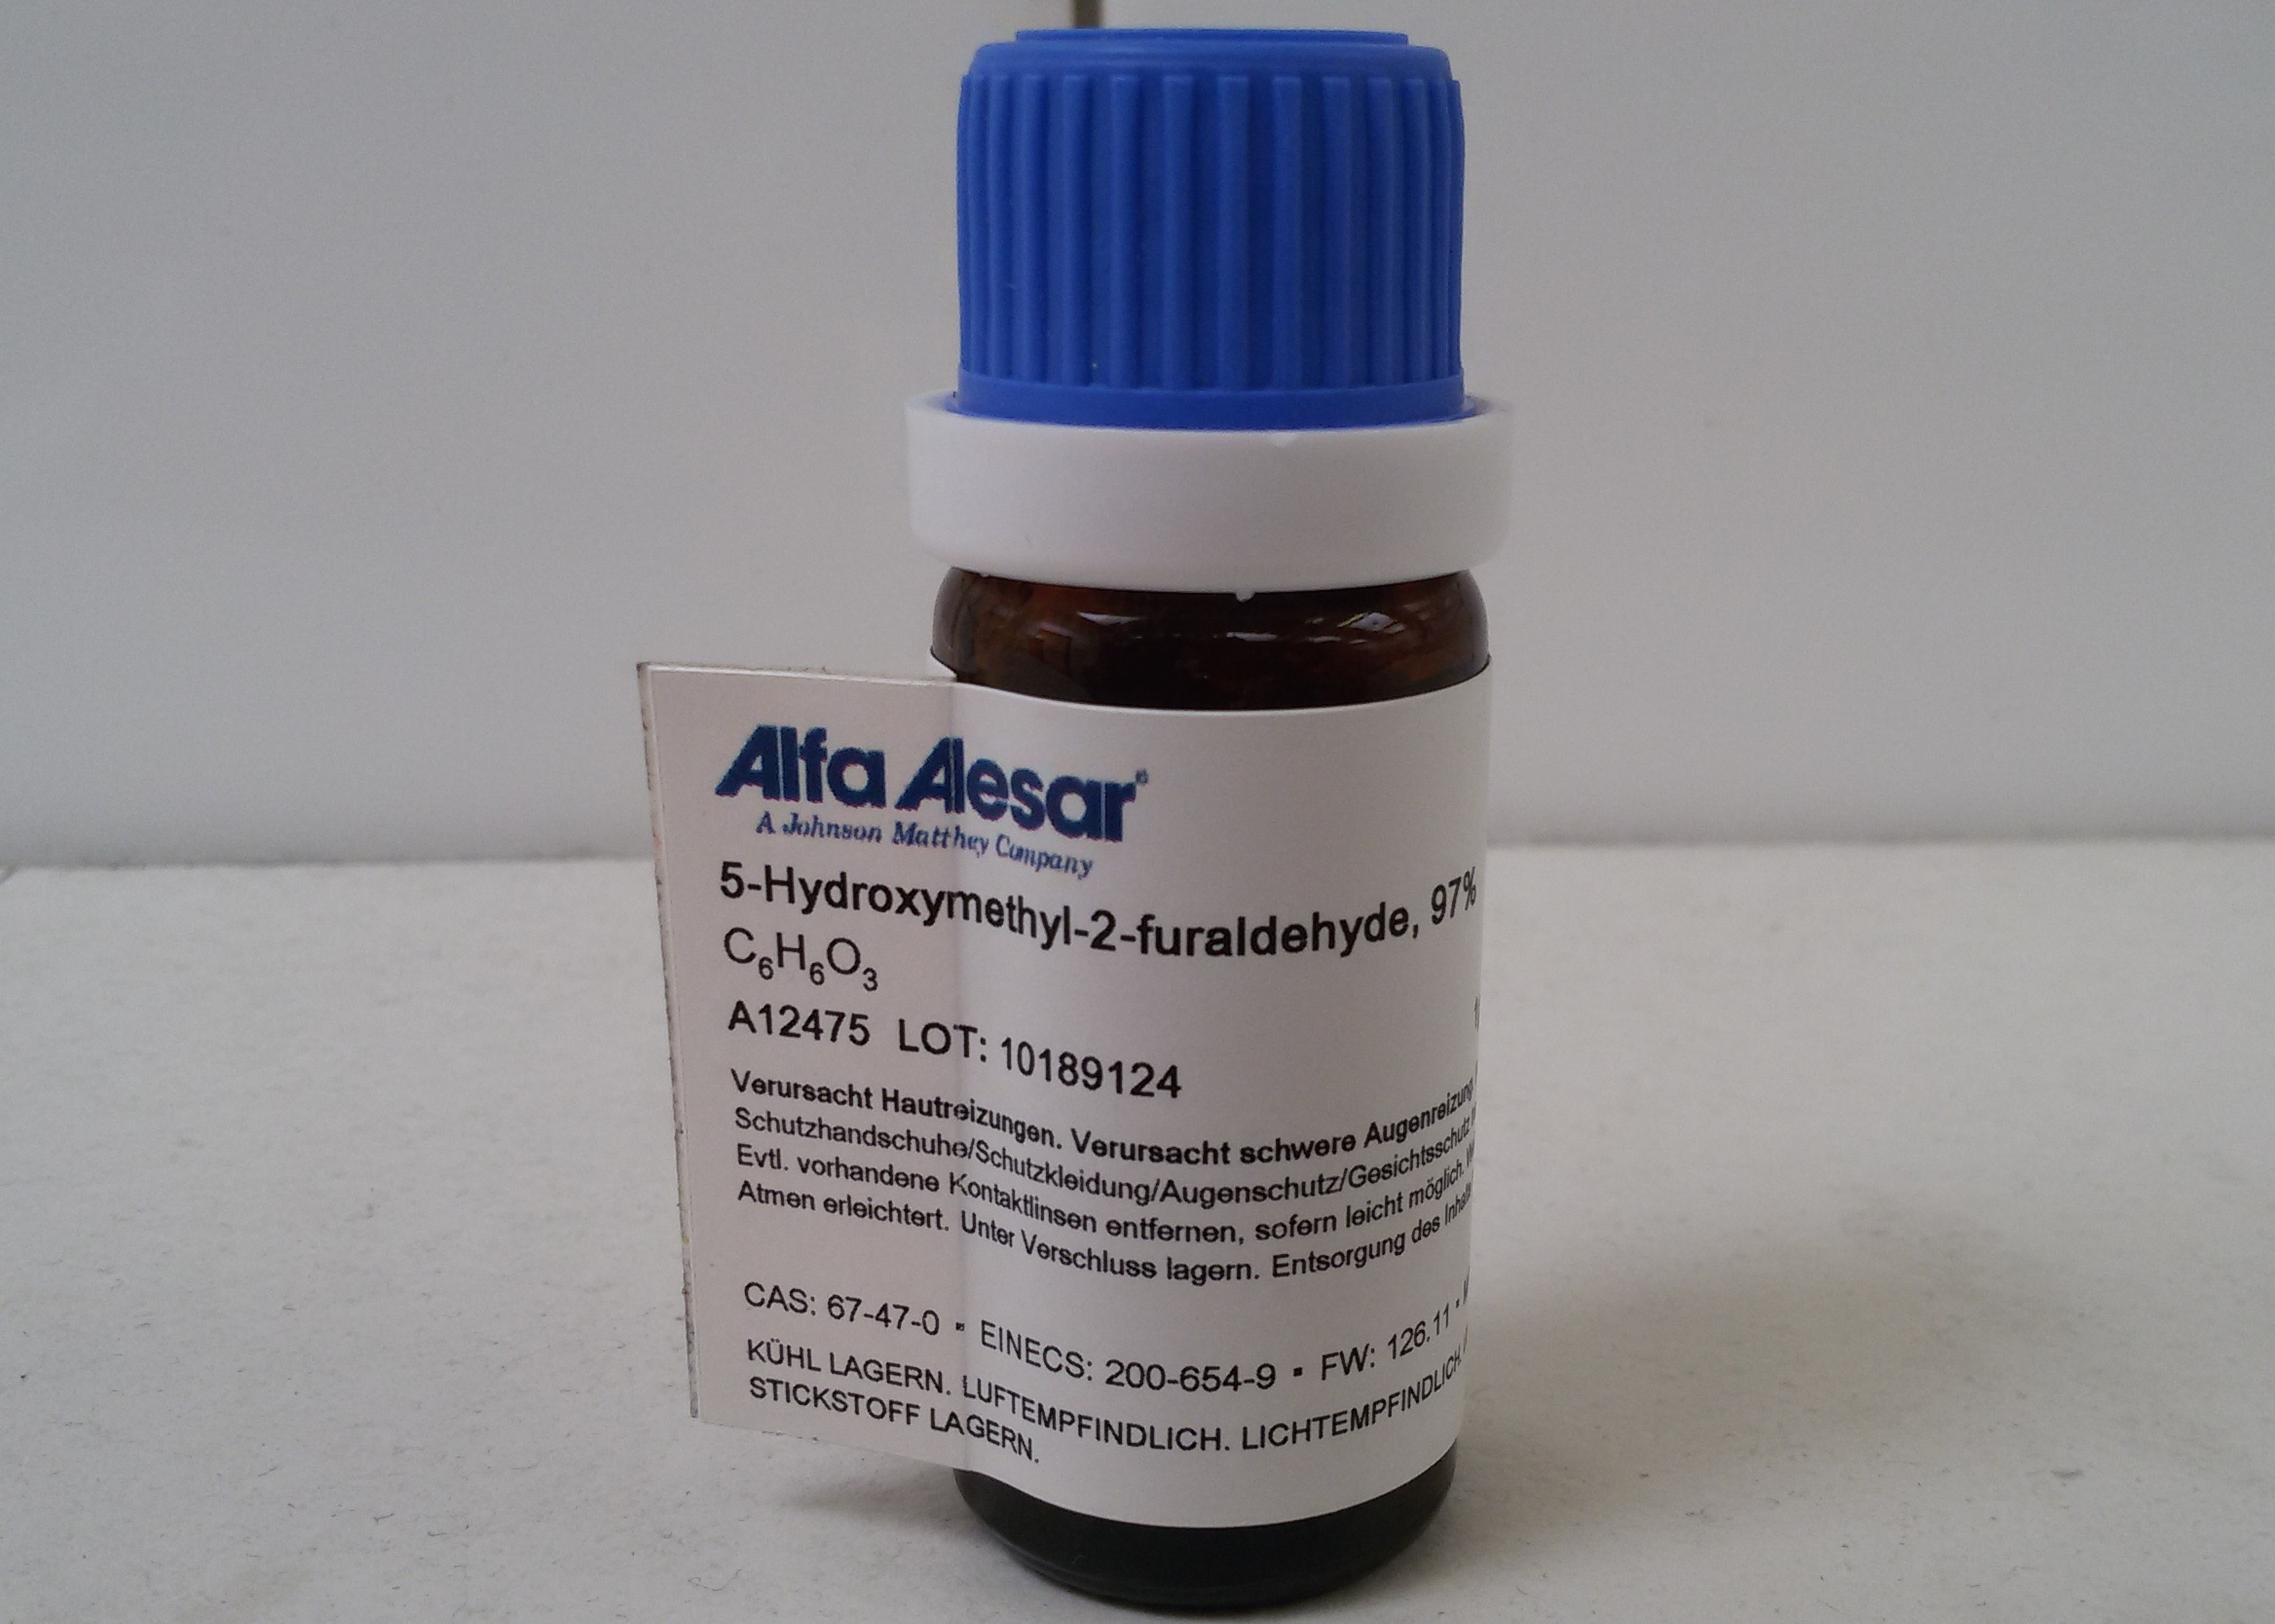
\includegraphics{../Bilder/20150504_140727.jpg}
    \caption{HMF-Reinsubstanz}
    \label{fig:HMF-Reinsubstanz}
\end{figure}
    
Die HMF-Reinsubstanz wird auf der Analysenwaage in einem Wägeschiffchen eingewogen, mit VE-Wasser in einen 10mL Messkolben überführt und bis zur Ringmarke aufgefüllt.\\
Einwaage SL1: 54,8mg\\
Einwaage SL2: 151,6mg\\
Aus den Einwaagen wird über die im Kapitel \ref{chap:Planung} verwendete Formel zur Konzentrationsberechnung die HMF-Konzentration der beiden Stammlösungen berechnet. Die Konzentration der Stammlösung 1 beträgt 5480mg/L und die Konzentration der Stammlösung 2 beträgt 15160mg/L.\\ 
Von beiden Stammlösungen wird je ein Milliliter in jeweils einen 100mL Messkolben überführt und mit VE-Wasser bis zur Ringmarke aufgefüllt. Somit ergibt sich für die Stammlösung 1.1 eine HMF-Konzentration von 54,8mg/L und für die Stammlösung 2.1 eine HMF-Konzentration von 151,6mg/L. 

    \section{Herstellung und Vermessung der Kalibrierlösungen}

    Für die Kalibrierlösungen werden aliquote Teile der beiden Stammlösungen 1.1 und 2.1 mit verschiedenen Vollpipetten in 50mL Messkolben abgefüllt und mit einigen Millilitern VE-Wasser vermischt. Die Berechnung der Volumina befindet sich im Kapitel \ref{chap:Planung}. Anschließend werden je 1mL Carrez-Lösung I und II mit einer Vollpipette hinzugefügt. Nach Durchmischen der Lösungen wird mit VE-Wasser bis zur Ringmarke aufgefüllt. Dabei fallen störende Matrixbestandteile als unlösliche Partikel aus.
    
    \begin{figure}[htbp]
      \centering
      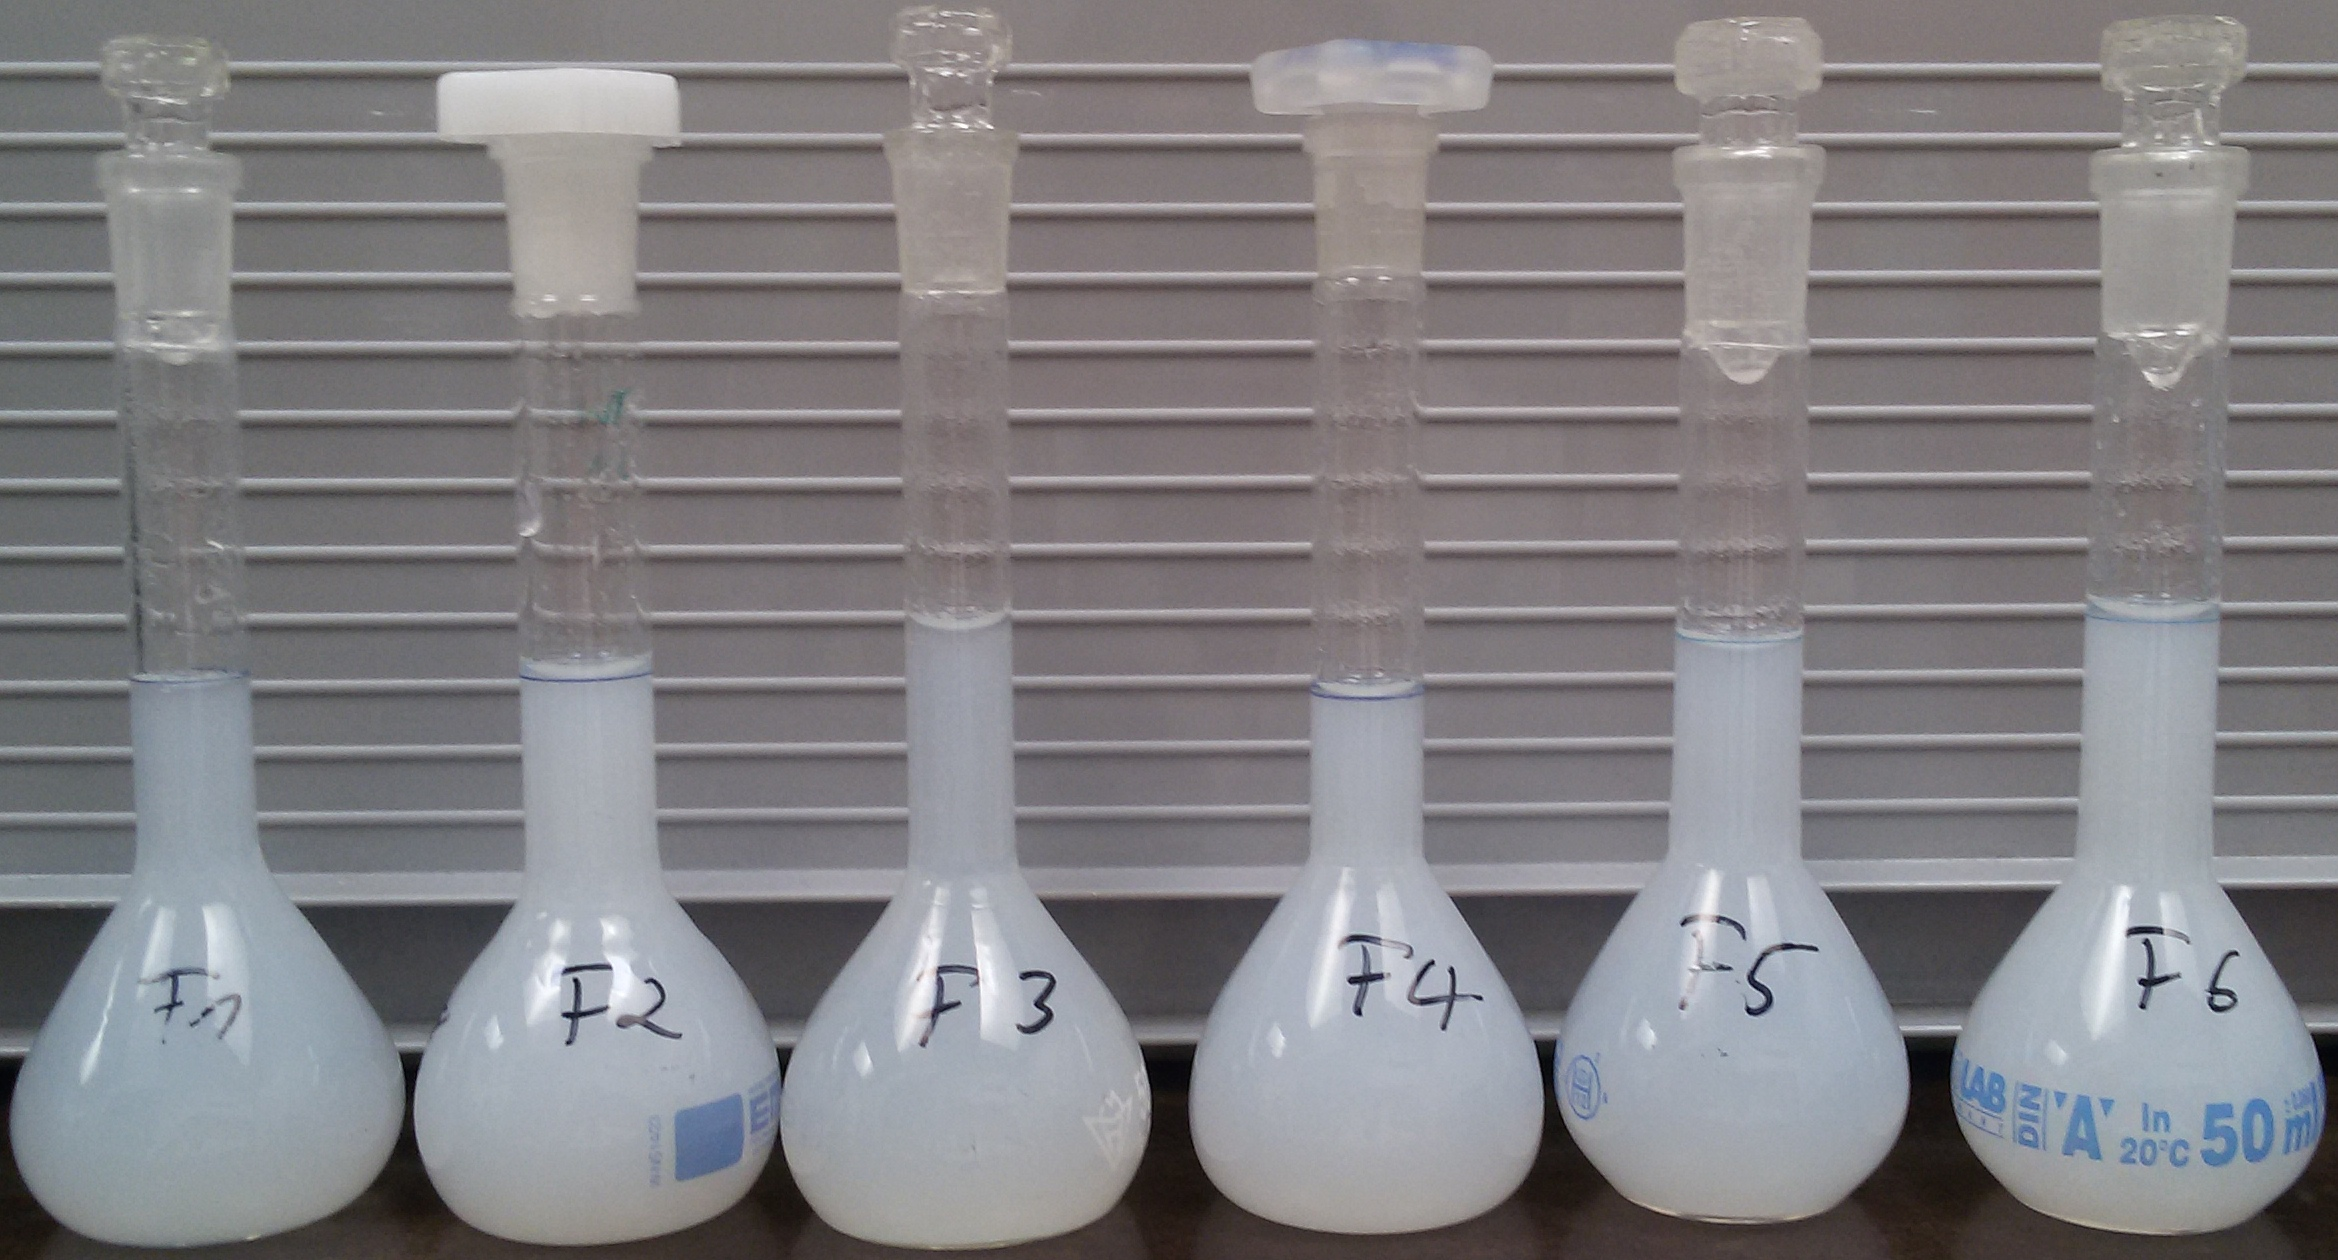
\includegraphics[width=1.00\textwidth]{../Bilder/20150424_155955.jpg}
      \caption{Kalibrierlösungen mit unlöslichen Partikeln}
      \label{fig:Partikel}
    \end{figure}
    
Die Lösungen werden über einen Faltenfilter filtriert, wobei die ersten 10mL Filtrat verworfen werden. Von dem restlichen Filtrat werden 2mL mit einer Vollpipette entnommen und in einen 10mL Messkolben überführt. In die Kolben werden außerdem jeweils 5mL p-Toluidinlösung und 1mL Barbitursäurelösung pipettiert. Von dem Filtrat der ersten Kalibrierlösung wird ebenfalls die Lösung für den Blindwert angesetzt. Hierbei werden 5mL p-Toluidinlösung zugegeben, aber anstelle der Barbitursäurelösung 1mL VE-Wasser zugesetzt. Zum Homogenisieren werden die Messkolben verschlossen und mehrmals invertiert. Da es sich bei der Farbreaktion um eine Zeitreaktion handelt, werden die Kalibrierlösungen und der Blindwert vor der Vermessung vier Minuten stehen gelassen. Danach müssen die Lösungen zügig vermessen werden, da der Farbkomplex nach dieser Zeit wieder zerfällt.\\
Mit der sechsten Kalibrierlösung wird die Wellenlänge des Absorptionsmaximums zwischen 200 und 800nm bestimmt. Der Ausdruck der Wellenlängenbestimmung ist in Anhang 1 zu finden.

\[
  \lambda_{max} = 550nm
\]

Dies entspricht der in der Literatur angegebenen Wellenlänge zur Vermessung des Farbkomplexes.~\cite{Winkler}\\
Die Kalibrierlösungen werden bei 550nm gegen den Blindwert vermessen und eine Kalibriergerade erstellt. Um Messfehler zu minimieren wird jede Kalibrierlösung dreimal gemessen.\\
In der nachfolgenden Tabelle \ref{tab:Kalibrierlösungen} sind die Kalibrierlösungen aufgelistet.

\begin{table}[htbp]
    \centering
    \caption{Kalibrierlösungen}
        \begin{tabular}{C{0.1\linewidth}|C{0.1\linewidth}|C{0.15\linewidth}|C{0.15\linewidth}|C{0.15\linewidth}|c} 
            Kalibrier-lösung & Stamm-lösung & Volumen Stamm-lösung\newline in mL & Massenkon-zentration berechnet\newline in mg/L & Massenanteil berechnet\newline in mg/kg & Extinktion\\
            \hline
            1 & 1.1 & 1 & 1,096 & 5,480 & 0,0400\\
            \hline
            2 & 1.2 & 1 & 3,032 & 15,16 & 0,1353\\
            \hline
            3 & 1.1 & 5 & 5,480 & 27,40 & 0,1687\\
            \hline
            4 & 1.1 & 10 & 10,96 & 54,80 & 0,3214\\
            \hline
            5 & 1.2 & 10 & 30,32 & 151,6 & 0,9453\\
            \hline
            6 & 1.2 & 20 & 60,64 & 303,2 & 1,8987\\
        \end{tabular}
        \label{tab:Kalibrierlösungen}
\end{table}

\begin{figure}[htbp]
    \centering
        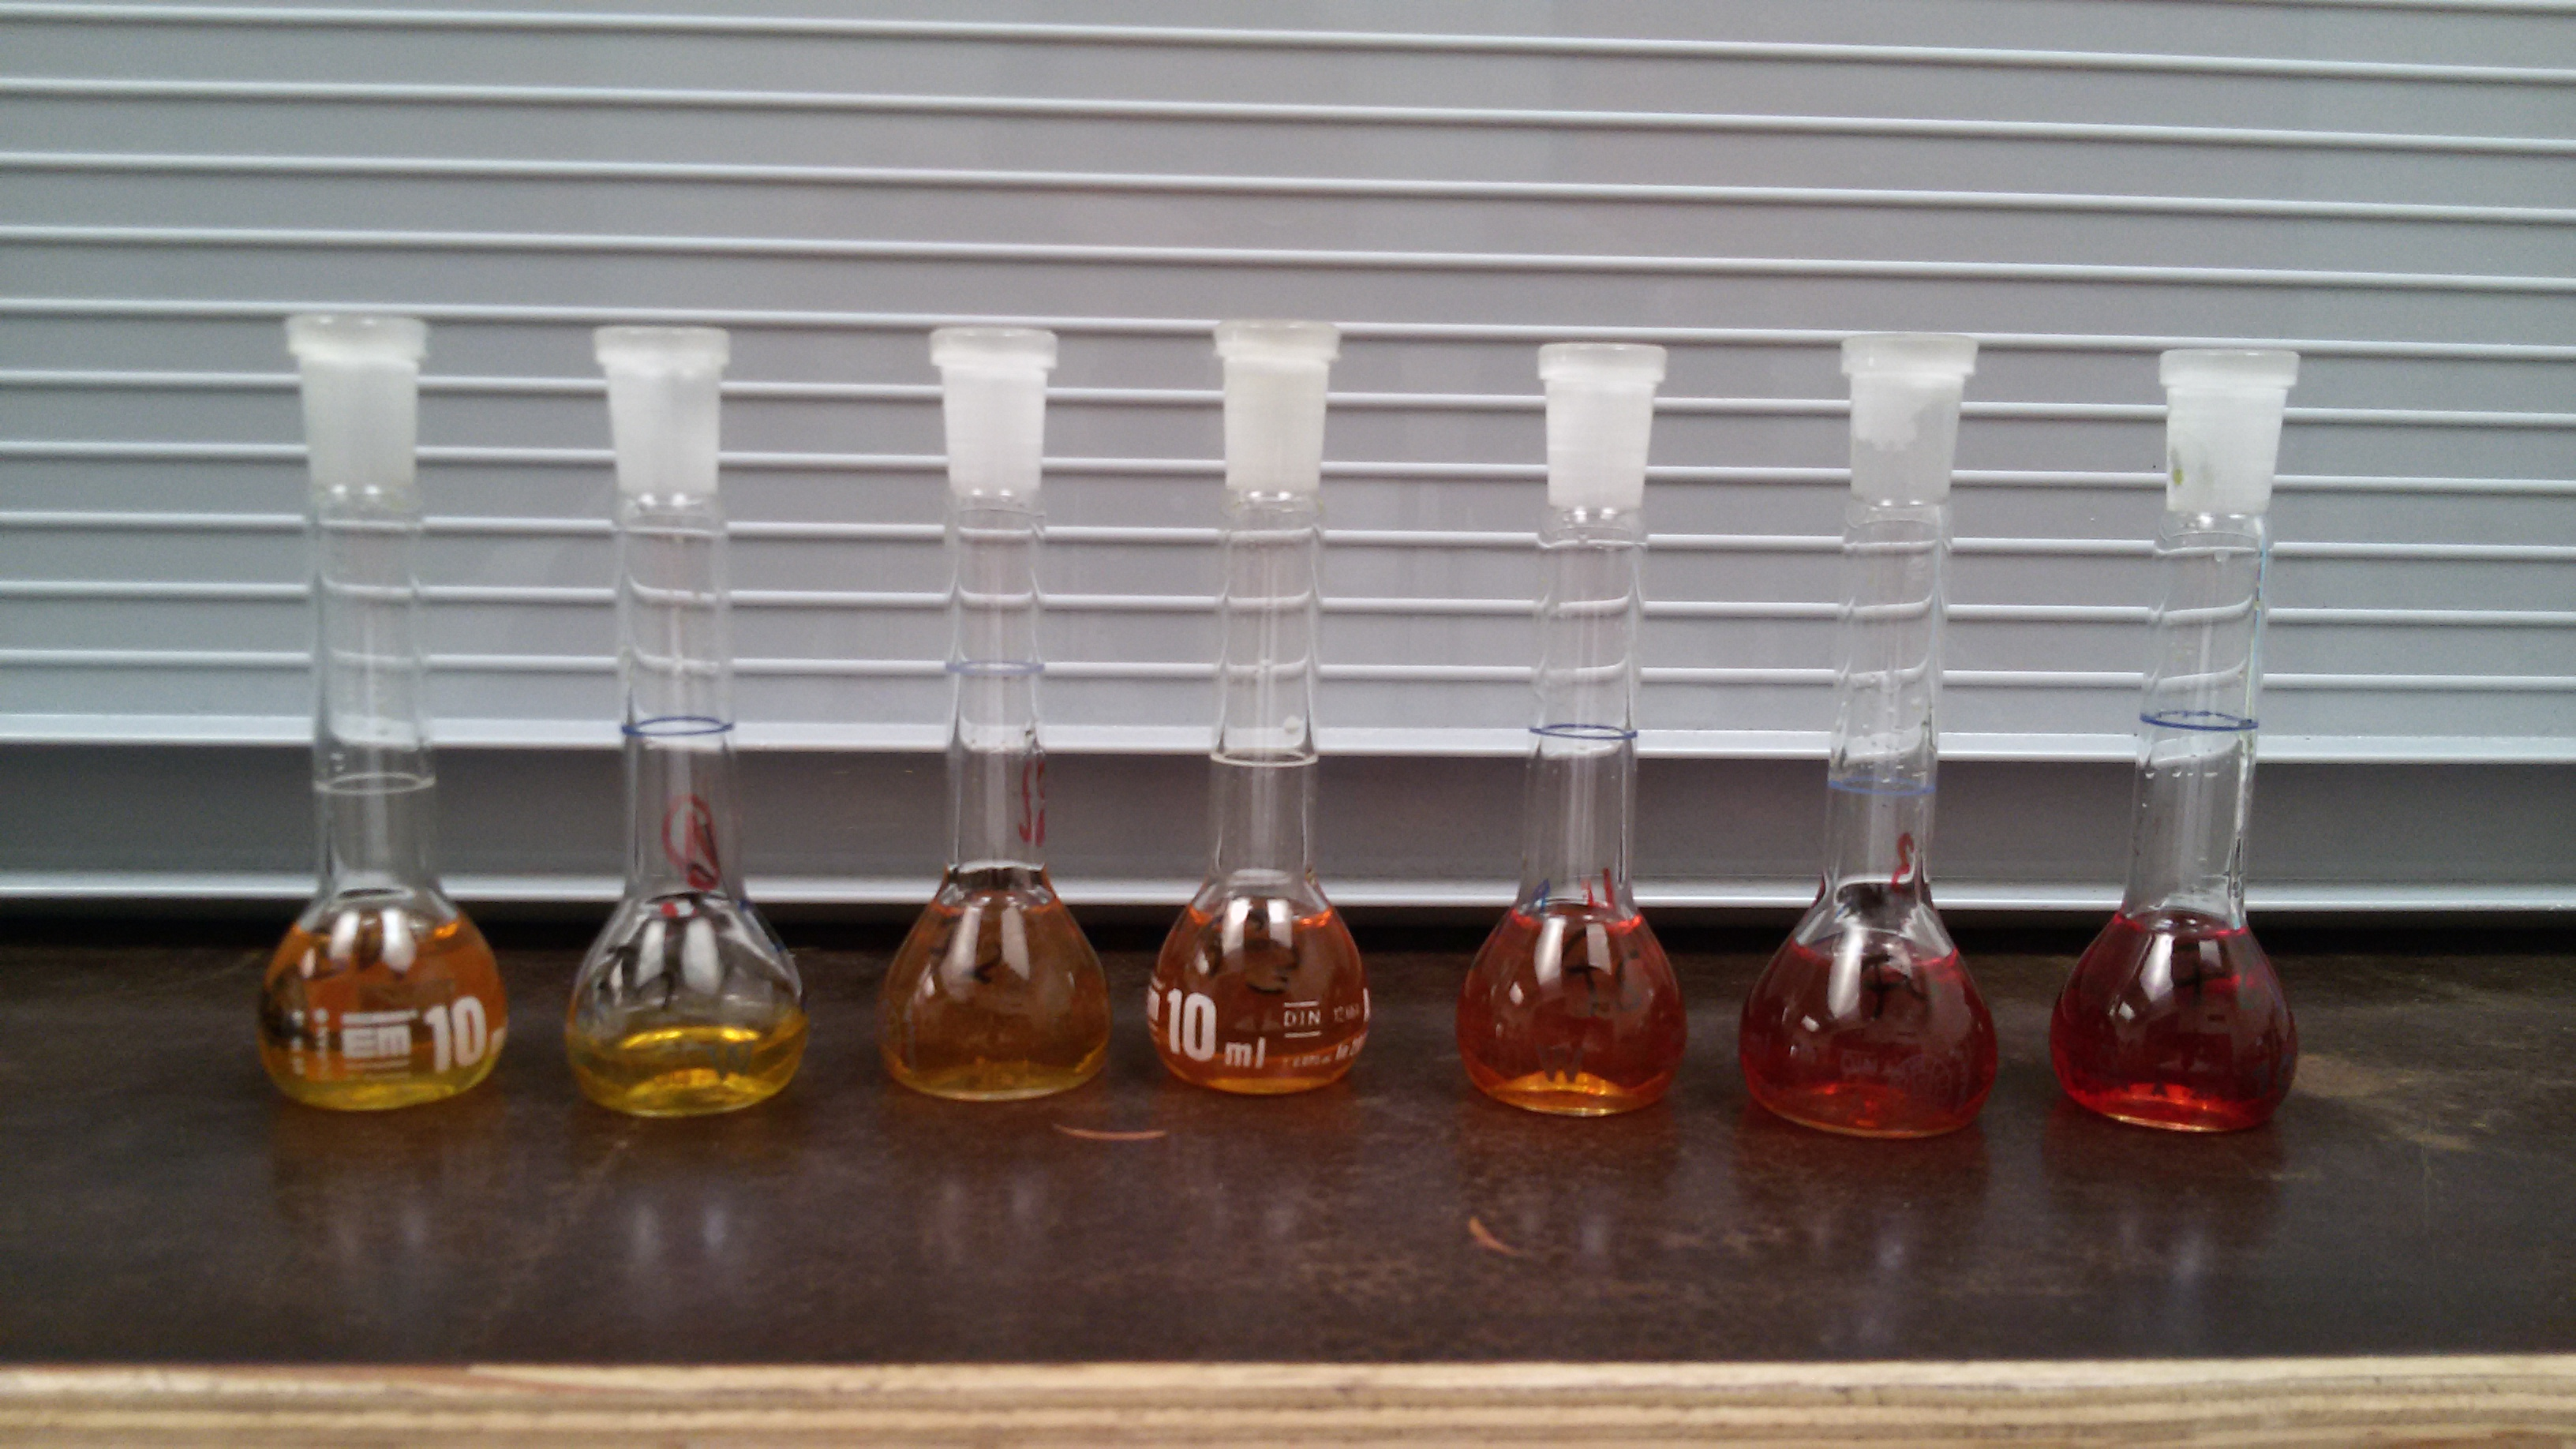
\includegraphics[width=1.00\textwidth]{../Bilder/20150424_172612.jpg}
    \caption{Kalibrierlösungen}
    \label{fig:Kalibrierlösungen}
\end{figure}


\section{Herstellung und Vermessung der Probelösungen}

Für die Probelösungen werden jeweils ca. 10g Probe in einen 50mL Messkolben eingewogen und in 20mL VE-Wasser gelöst. Die folgende Tabelle \ref{tab:Probeneinwaage} enthält die Lagertemperatur und die Einwaage der einzelnen Proben. 

\begin{table}[htbp]
    \centering
    \caption{Probeneinwaage}
        \begin{tabular}{c|c|c} 
            Probennummer & Lagertemperatur in $^\circ$C & Einwaage in g\\
            \hline
            1 & 25 & 10,2926\\
            \hline
            1 & 60 & 11,0590\\
            \hline
            2 & 25 & 10,2548\\
            \hline
            2 & 60 & 10,0891\\
            \hline
            3 & 25 & 11,3998\\
            \hline
            3 & 60 & 10,2277\\
            \hline
            4 & 25 & 9,9125\\
            \hline
            4 & 60 & 10,0411\\
            \hline
            5 & 25 & 10,0203\\
            \hline
            5 & 60 & 10,2194\\
            \hline
            6 & 25 & 10,0776\\
            \hline
            6 & 60 & 10,0968\\
            \hline
            7 & 25 & 10,4448\\
            \hline
            8 & 25 & 10,4160\\
            \hline
            9 & 25 & 10,1488\\
            \hline
            10 & 25 & 9,9153\\
        \end{tabular}
    \label{tab:Probeneinwaage}
\end{table}

Jeder Probelösung werden je 1mL Carrez-Lösung I und II zugesetzt und die Messkolben nach dem Homogenisieren mit VE-Wasser bis zur Ringmarke aufgefüllt. Die ausgefallenen Partikel werden über Faltenfilter abfiltriert.

\begin{figure}[htbp]
    \centering
        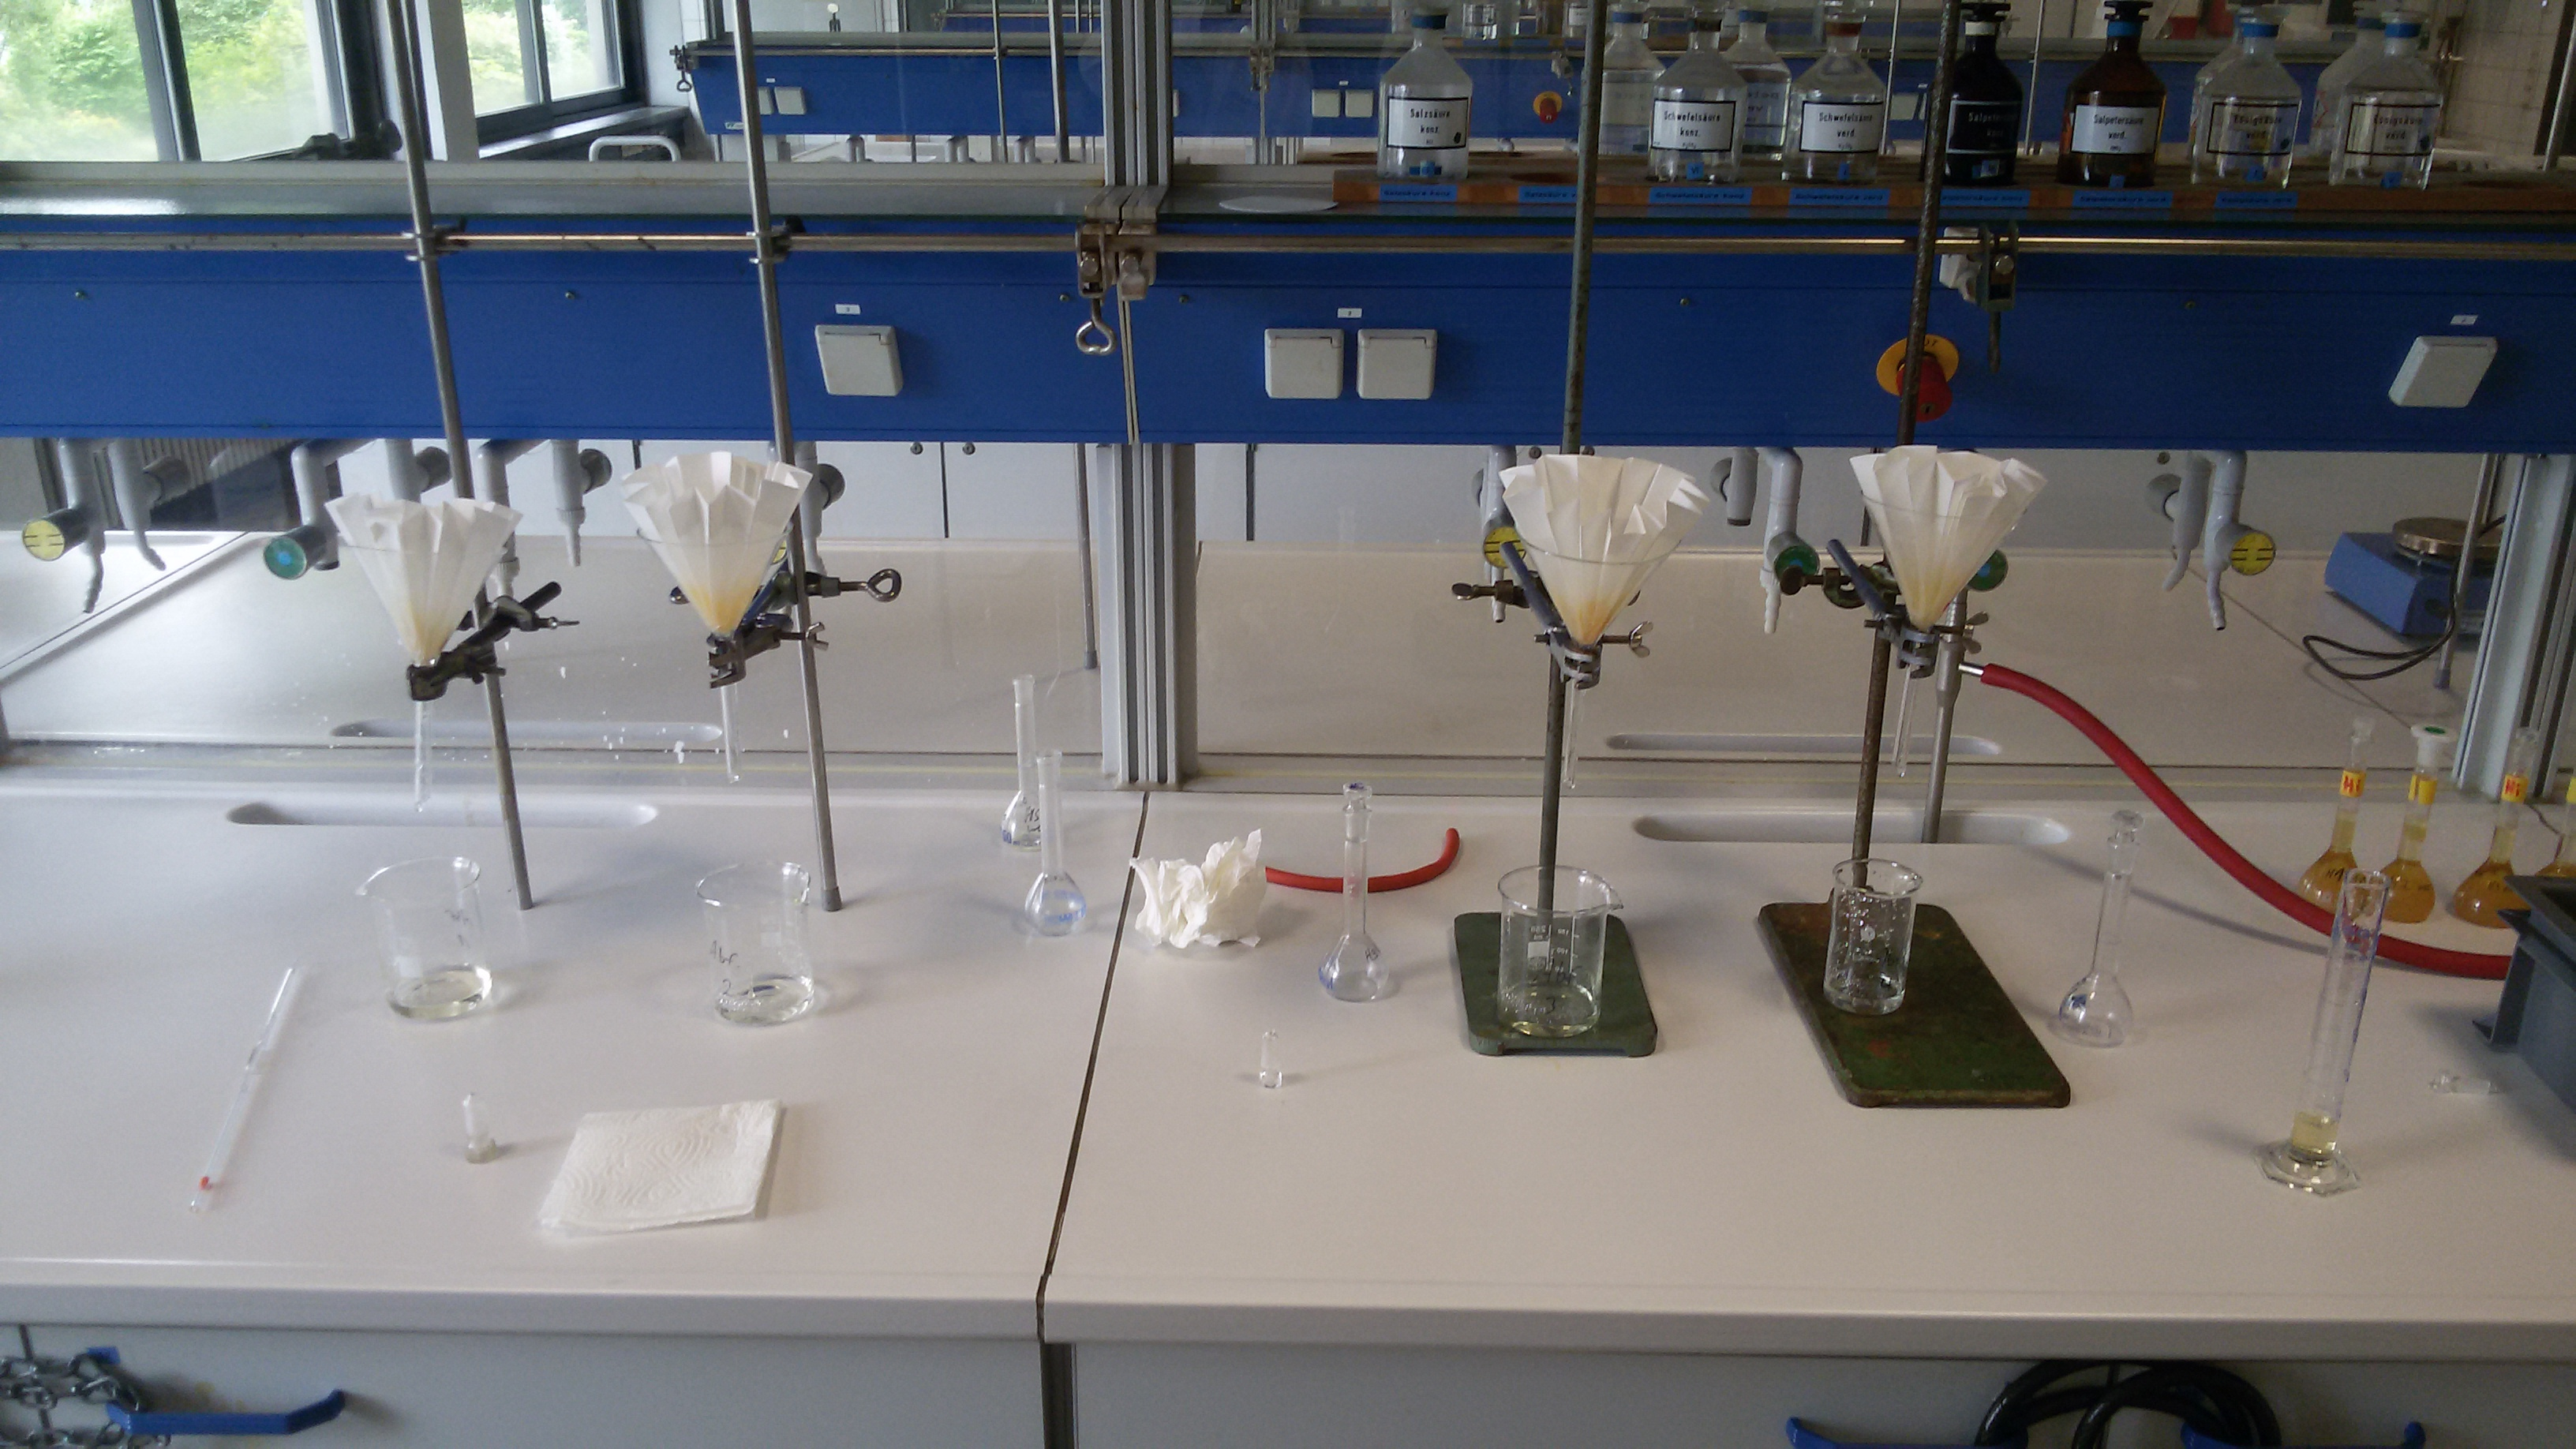
\includegraphics[width=1.00\textwidth]{../Bilder/20150427_131648.jpg}
    \caption{Filtration der Proben}
    \label{fig:Filtration}
\end{figure}

Dabei werden die ersten 10mL des Filtrats verworfen. Von dem Filtrat werden mit einer Vollpipette jeweils zweimal 2mL entnommen und in zwei 10mL Messkolben überführt. In einem Messkolben wird der Blindwert angesetzt, im anderen die zu vermessende Probe. In beide Messkolben werden je 5mL p-Toluidinlösung hinzugefügt. Mit einer 1mL Vollpipette wird dem Blindwert 1mL VE-Wasser zugegeben und der Probelösung 1mL Barbitursäurelösung. Beide Messkolben bleiben nach dem Homogenisieren für vier Minuten stehen. Die Messung der Probe erfolgt danach bei 550nm gegen den jeweiligen Blindwert. Die Proben werden jeweils dreimal vermessen um Messfehler möglichst gering zu halten.
\begin{figure}[htbp]
    \centering
        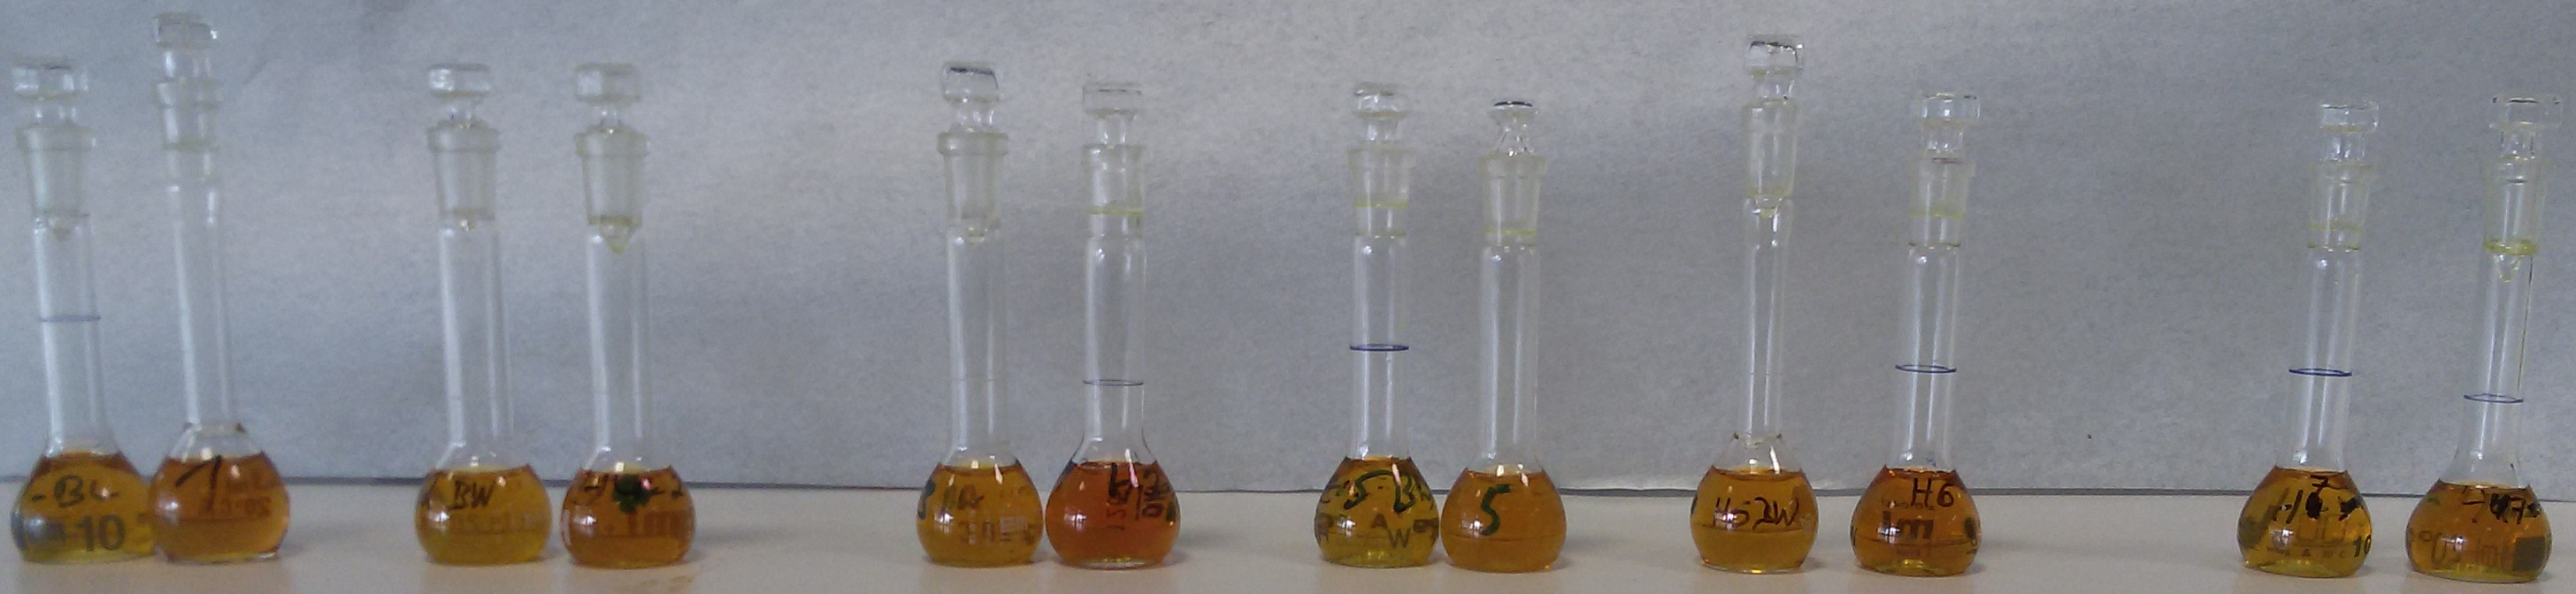
\includegraphics[width=1.00\textwidth]{../Bilder/20150427_140221(0).jpg}
    \caption{Probenauswahl mit Blindwerten}
    \label{fig:Probenauswahl}
\end{figure}

\newpage
\section{Mehrfachbestimmung und Aufstockung einer Probe}

Für eine Mehrfachbestimmung wird die Honigprobe 3 am zweiten Praktikumstag einmal und am dritten Praktikumstag sechsmal eingewogen, wie oben beschrieben mit Reaktionslösungen versetzt und anschließend vermessen. Außerdem werden zwei zusätzliche Einwaagen der Honigprobe 3 einmal mit 10mL der Stammlösung 1.1 und einmal mit 5mL der Stammlösung 2.1 versetzt und so der HMF-Gehalt aufgestockt. Diese beiden Proben werden ebenfalls wie oben beschrieben behandelt und vermessen. Die Einwaagen sind in folgender Tabelle \ref{tab:Probeneinwaage Mehrfachbestimmung + Aufstockungen} aufgeführt:
\begin{table}[htbp]
    \centering
    \caption{Probeneinwaage Mehrfachbestimmung + Aufstockungen}
        \begin{tabular}{c|c|c} 
            Probennummer & Lagertemperatur in $^\circ$C & Einwaage in g\\
            \hline
            3.1 & 25 & 10,323\\
            \hline
            3.2 & 25 & 10,358\\
            \hline
            3.3 & 25 & 10,199\\
            \hline
            3.4 & 25 & 10,835\\
            \hline
            3.5 & 25 & 10,414\\
            \hline
            3.6 & 25 & 10,286\\
            \hline
            3.7 Aufst.1 & 25 & 10,483\\
            \hline
            3.8 Aufst.2 & 25 & 10,365\\
        \end{tabular}
    \label{tab:Probeneinwaage Mehrfachbestimmung + Aufstockungen}
\end{table}
